\documentclass[11pt,a4paper]{article}
\usepackage[margin=2.5cm]{geometry}
\usepackage{amsmath,amssymb,amsthm}
\usepackage{bm}
\usepackage{graphicx}
\usepackage{xcolor}
\usepackage{tcolorbox}
\usepackage{hyperref}
\usepackage{tikz}
\usetikzlibrary{matrix,arrows.meta,positioning}

\definecolor{darkblue}{RGB}{0,51,102}
\definecolor{accent}{RGB}{200,50,50}

\hypersetup{colorlinks=true,linkcolor=darkblue,citecolor=darkblue}

\theoremstyle{definition}
\newtheorem{definition}{Definition}
\newtheorem{theorem}{Theorem}
\newtheorem{proposition}{Proposition}
\newtheorem{remark}{Remark}

\title{\textbf{Eigenvector Equivalence of the\\Two-Phase PageRank Model}\\[6pt]
\large From Power Iteration to the Google Matrix}
\author{Two-Phase PageRank Project}
\date{\today}

\begin{document}
\maketitle

\begin{abstract}
This document rigorously derives how the Two-Phase PageRank power iteration
can be reformulated as a standard eigenvector problem by absorbing the
teleportation vector $\bm{E}_{2N}$ into the transition matrix $M_{2N}$,
forming the \emph{Google Matrix} $\widetilde{M}$.  We prove that the
stationary distribution $\bm{v}^*$ is the unique principal eigenvector of
$\widetilde{M}$ with eigenvalue $\lambda=1$, and explain why power iteration
is the preferred computational method.
\end{abstract}

\tableofcontents
\vspace{1em}

%======================================================================
\section{The Two-Phase PageRank Formulation}
%======================================================================

\subsection{\texorpdfstring{The $2N \times 2N$ Transition Matrix}{The 2N x 2N Transition Matrix}}

Let the road network have $N$ directed links.  Our Two-Phase model constructs
a block matrix of dimension $2N \times 2N$:

\begin{equation}\label{eq:M2N}
M_{2N} =
\begin{pmatrix}
(1-\beta)\,P_{\text{up}} & \beta\,I_N \\[4pt]
\bm{0}_{N\times N} & P_{\text{down}}
\end{pmatrix}
\end{equation}

where:
\begin{itemize}
  \item $P_{\text{up}}$ is the \textbf{upstream transition matrix} with
        travel-time self-loops: a vehicle on link $i$ either stays
        (self-loop weight $w_i = \mu \cdot \ell_i / s_i$) or moves to an
        upstream neighbor.
  \item $P_{\text{down}}$ is the \textbf{downstream transition matrix}:
        uniform splitting among downstream neighbors.
  \item $\beta \in (0,1)$ is the \textbf{phase-switch probability}: at each
        step, a vehicle in the upstream phase switches to the downstream
        phase with probability $\beta$.
  \item $I_N$ is the $N \times N$ identity matrix (the phase-switch landing).
\end{itemize}

\subsection{The Teleportation Vector}

The teleportation (personalization) vector encodes the ground-truth traffic
distribution derived from GPS observations:

\begin{equation}\label{eq:E2N}
\bm{E}_{2N} =
\begin{pmatrix}
\bm{E}_N \\[2pt]
\bm{0}_N
\end{pmatrix}
\in \mathbb{R}^{2N}, \qquad
\sum_{i=1}^{N} E_N[i] = 1, \quad E_N[i] \geq 0.
\end{equation}

Vehicles are always \emph{teleported} (injected) into the upstream phase,
never directly into the downstream phase.

\subsection{The Power Iteration}

The stationary distribution $\bm{v}^*$ is computed by iterating:

\begin{equation}\label{eq:power}
\boxed{
\bm{v}^{(t+1)} = d \cdot M_{2N}^T \, \bm{v}^{(t)}
                + (1-d) \cdot \bm{E}_{2N}
}
\end{equation}

where $d \in (0,1)$ is the \textbf{damping factor} (we use $d = 0.80$).
At convergence, $\bm{v}^* = \lim_{t\to\infty} \bm{v}^{(t)}$.

%======================================================================
\section{\texorpdfstring{Absorbing $\bm{E}_{2N}$ into the Matrix}{Absorbing E\_2N into the Matrix}}
%======================================================================

\subsection{Key Observation}

The teleportation term $(1-d)\,\bm{E}_{2N}$ does not depend on $\bm{v}$.
It is a constant additive correction applied at every iteration.  We can
eliminate it by constructing a single matrix that encodes both the
transition dynamics \emph{and} the teleportation.

\subsection{The Google Matrix Construction}

\begin{definition}[{Google Matrix}]
Define the \textbf{Google Matrix} $\widetilde{M} \in \mathbb{R}^{2N \times 2N}$ as:
\begin{equation}\label{eq:google}
\boxed{
\widetilde{M} \;=\; d \cdot M_{2N}^T
\;+\; (1-d) \cdot \bm{E}_{2N}\,\bm{1}^T
}
\end{equation}
where $\bm{1} \in \mathbb{R}^{2N}$ is the all-ones vector.
\end{definition}

\begin{remark}
The term $\bm{E}_{2N}\,\bm{1}^T$ is a \textbf{rank-1 matrix} of size
$2N \times 2N$.  Its $(i,j)$-th entry is simply $E_{2N}[i]$, regardless
of~$j$.  This means that from \emph{every} state $j$, there is a
probability $(1-d)\cdot E_{2N}[i]$ of teleporting to state~$i$.
\end{remark}

\subsection{Block-by-Block Expansion}

A natural question arises: \emph{can we simply place $\bm{E}_{2N}$ inside the
original matrix $M_{2N}$ to form a single matrix?}  The answer requires
careful expansion.  The teleportation does \textbf{not} simply replace one
block---it adds a rank-1 correction that spreads across the entire top half
of the matrix.

\medskip
\noindent\textbf{Step 1: Expand the outer product.}
Recall that $\bm{E}_{2N} = (\bm{E}_N,\, \bm{0}_N)^T$.  The rank-1 matrix
$\bm{E}_{2N}\bm{1}^T$ therefore has the block structure:
\begin{equation}\label{eq:outerblock}
\bm{E}_{2N}\,\bm{1}^T
= \begin{pmatrix} \bm{E}_N \\ \bm{0}_N \end{pmatrix}
  \begin{pmatrix} \bm{1}_N^T & \bm{1}_N^T \end{pmatrix}
= \begin{pmatrix}
    \bm{E}_N\,\bm{1}_N^T & \bm{E}_N\,\bm{1}_N^T \\[4pt]
    \bm{0}_{N\times N}    & \bm{0}_{N\times N}
  \end{pmatrix}
\end{equation}

Here $\bm{E}_N\,\bm{1}_N^T$ is an $N \times N$ matrix where \emph{every column
is identical}: column $j$ equals $\bm{E}_N$ for all $j = 1, \dots, N$.

\begin{remark}
Because $\bm{E}_{2N}$ has zeros in its bottom $N$ entries, the rank-1
correction only affects the \textbf{top two blocks} of the Google Matrix.  The
bottom two blocks remain unchanged.
\end{remark}

\medskip
\noindent\textbf{Step 2: Expand $M_{2N}^T$.}
Transposing the original block matrix~\eqref{eq:M2N}:
\begin{equation}\label{eq:M2Ntranspose}
M_{2N}^T =
\begin{pmatrix}
(1-\beta)\,P_{\text{up}}^T & \bm{0}_{N\times N} \\[4pt]
\beta\,I_N                 & P_{\text{down}}^T
\end{pmatrix}
\end{equation}

Note how the blocks move: $\beta I_N$ shifts from top-right to bottom-left,
and the zero block shifts from bottom-left to top-right.

\medskip
\noindent\textbf{Step 3: Combine into the Google Matrix.}
Substituting~\eqref{eq:M2Ntranspose} and~\eqref{eq:outerblock} into the
Google Matrix definition~\eqref{eq:google}:

\begin{equation}\label{eq:googleblocks}
\boxed{
\widetilde{M} =
\begin{pmatrix}
d(1-\beta)\,P_{\text{up}}^T + {\color{accent}(1-d)\,\bm{E}_N\bm{1}_N^T}
  & {\color{accent}(1-d)\,\bm{E}_N\bm{1}_N^T} \\[6pt]
d\beta\, I_N
  & d\,P_{\text{down}}^T
\end{pmatrix}
}
\end{equation}

The terms in {\color{accent}red} are the contributions from the teleportation
vector.  Notice that:
\begin{itemize}
  \item The teleportation is \textbf{added to} the top-left block (not
        replacing $P_{\text{up}}^T$).
  \item The top-right block, which was $\bm{0}$ in $M_{2N}^T$, is now
        \textbf{entirely} the teleportation matrix
        $(1-d)\,\bm{E}_N\bm{1}_N^T$.
  \item The bottom-left block ($d\beta I_N$) is \textbf{unchanged}---the
        phase-switch mechanism is preserved.
  \item The bottom-right block ($d P_{\text{down}}^T$) is
        \textbf{unchanged}---the downstream dynamics are preserved.
\end{itemize}

\medskip
\noindent\textbf{Physical interpretation of each block:}

\begin{center}
\renewcommand{\arraystretch}{1.4}
\begin{tabular}{|c|c|c|}
\hline
\textbf{Block} & \textbf{From $\to$ To} & \textbf{Meaning} \\
\hline
Top-Left & Up $\to$ Up &
\begin{minipage}{6.5cm}\small
  Vehicle follows upstream neighbors \emph{or} teleports
  back to a high-traffic upstream link.
\end{minipage} \\
\hline
Top-Right & Down $\to$ Up &
\begin{minipage}{6.5cm}\small
  Vehicle in the downstream phase teleports directly
  to a high-traffic upstream link (with probability $1-d$).
\end{minipage} \\
\hline
Bottom-Left & Up $\to$ Down &
\begin{minipage}{6.5cm}\small
  Vehicle switches from upstream to downstream phase
  (probability $d\beta$). No teleportation here.
\end{minipage} \\
\hline
Bottom-Right & Down $\to$ Down &
\begin{minipage}{6.5cm}\small
  Vehicle follows downstream neighbors.
  No teleportation here.
\end{minipage} \\
\hline
\end{tabular}
\end{center}

\medskip
\noindent\textbf{Sparsity consequences.}
The original $M_{2N}$ is highly sparse ($\sim$200K nonzero entries out of
$4N^2 \approx 4 \times 10^{10}$ possible entries).  The Google Matrix
$\widetilde{M}$ is \textbf{not sparse}: the top-left and top-right blocks
each contain $N^2 \approx 10^{10}$ nonzero entries (because
$\bm{E}_N\bm{1}_N^T$ is dense).

\begin{tcolorbox}[colback=red!5,colframe=accent,title=Why We Cannot Store $\widetilde{M}$]
For $N = 99{,}716$ links:
\begin{itemize}
  \item Top-left block: $N^2 = 9.94 \times 10^9$ entries $\times$ 8 bytes $\approx$ \textbf{74 GB}
  \item Top-right block: $N^2 = 9.94 \times 10^9$ entries $\times$ 8 bytes $\approx$ \textbf{74 GB}
  \item Total: $\approx$ \textbf{148 GB} of dense storage
\end{itemize}
This is why we use power iteration: it computes the same eigenvector by
keeping $M_{2N}$ sparse and adding $\bm{E}_{2N}$ as a cheap $O(2N)$ vector
operation at each step.
\end{tcolorbox}

\subsection{Derivation of Equivalence}

\begin{theorem}[{Eigenvector Equivalence}]\label{thm:equiv}
The fixed point of the power iteration~\eqref{eq:power} is the principal
eigenvector of $\widetilde{M}$ with eigenvalue $\lambda = 1$:
\[
\bm{v}^* = \widetilde{M}\,\bm{v}^*.
\]
\end{theorem}

\begin{proof}
At convergence, $\bm{v}^{(t+1)} = \bm{v}^{(t)} = \bm{v}^*$.
Substituting into~\eqref{eq:power}:
\begin{align}
\bm{v}^* &= d \cdot M_{2N}^T\,\bm{v}^*
           + (1-d) \cdot \bm{E}_{2N}. \label{eq:fixed}
\end{align}

Since $\bm{v}^*$ is a probability vector, $\bm{1}^T \bm{v}^* = 1$.
Therefore:
\begin{align}
(1-d) \cdot \bm{E}_{2N}
&= (1-d) \cdot \bm{E}_{2N} \cdot 1 \notag \\
&= (1-d) \cdot \bm{E}_{2N} \cdot (\bm{1}^T \bm{v}^*) \notag \\
&= \bigl[(1-d) \cdot \bm{E}_{2N}\,\bm{1}^T\bigr]\,\bm{v}^*. \label{eq:rank1}
\end{align}

Substituting~\eqref{eq:rank1} into~\eqref{eq:fixed}:
\begin{align}
\bm{v}^*
&= d \cdot M_{2N}^T\,\bm{v}^*
 + \bigl[(1-d) \cdot \bm{E}_{2N}\,\bm{1}^T\bigr]\,\bm{v}^* \notag \\
&= \bigl[\underbrace{d \cdot M_{2N}^T
 + (1-d) \cdot \bm{E}_{2N}\,\bm{1}^T}_{\widetilde{M}}\bigr]\,\bm{v}^* \notag \\
&= \widetilde{M}\,\bm{v}^*. \qedhere
\end{align}
\end{proof}

%======================================================================
\section{\texorpdfstring{Properties of $\widetilde{M}$}{Properties of M-tilde}}
%======================================================================

\begin{proposition}[{$\widetilde{M}$ is Column-Stochastic}]\label{prop:stochastic}
Every column of $\widetilde{M}$ sums to~1.
\end{proposition}

\begin{proof}
For any column $j$:
\begin{align}
\bm{1}^T \widetilde{M}_{:,j}
&= d \cdot \bm{1}^T (M_{2N}^T)_{:,j}
 + (1-d) \cdot \bm{1}^T (\bm{E}_{2N}\,\bm{1}^T)_{:,j} \notag \\
&= d \cdot \underbrace{\sum_i M_{2N}[j,i]}_{=\,1\text{ (row-stochastic)}}
 + (1-d) \cdot \underbrace{\sum_i E_{2N}[i]}_{=\,1} \notag \\
&= d + (1-d) = 1. \qedhere
\end{align}
\end{proof}

\begin{proposition}[{Unique Stationary Distribution}]\label{prop:unique}
$\widetilde{M}$ has a unique eigenvector with eigenvalue $\lambda = 1$.
\end{proposition}

\begin{proof}
The rank-1 perturbation $(1-d)\,\bm{E}_{2N}\bm{1}^T$ has all strictly
positive entries (since $E_N[i] > 0$ for all $i$ after Laplace smoothing
and $1-d > 0$).  Therefore $\widetilde{M}$ is a \textbf{primitive}
stochastic matrix (every entry is strictly positive in at least one power).
By the \textbf{Perron--Frobenius theorem}, a primitive stochastic matrix
has a unique stationary distribution, corresponding to the unique
eigenvector with eigenvalue $\lambda = 1$.
\end{proof}

%======================================================================
\section{Why Power Iteration is Used Instead}
%======================================================================

Although $\bm{v}^*$ is theoretically the principal eigenvector of
$\widetilde{M}$, computing it via eigendecomposition is impractical:

\begin{center}
\renewcommand{\arraystretch}{1.3}
\begin{tabular}{lcc}
\hline
\textbf{Property} & \textbf{Eigendecomposition} & \textbf{Power Iteration} \\
\hline
Matrix form & Dense $\widetilde{M}$ & Sparse $M_{2N}$ + vector $\bm{E}_{2N}$ \\
Memory & $O(4N^2)$ entries & $O(\text{nnz}(M_{2N}) + 2N)$ \\
Time complexity & $O((2N)^3)$ & $O(k \cdot \text{nnz}(M_{2N}))$ \\
\hline
\multicolumn{3}{l}{\small For $N = 99{,}716$:} \\
Memory & $\approx$ 300 GB & $\approx$ 50 MB \\
Time & $\approx$ years & $\approx$ 3 seconds \\
Iterations & 1 (but cubic) & $k \approx 40$ \\
\hline
\end{tabular}
\end{center}

\begin{tcolorbox}[colback=blue!5,colframe=darkblue,title=Key Insight]
Power iteration \textbf{is} the eigenvector computation---it is simply the
most efficient algorithm for finding the principal eigenvector of a matrix
that is the sum of a large sparse matrix and a small rank-1 correction.
Each iteration computes:
\[
\bm{v}^{(t+1)} = \underbrace{d \cdot M_{2N}^T \bm{v}^{(t)}}_{\text{sparse
matvec: } O(\text{nnz})} + \underbrace{(1-d) \cdot
\bm{E}_{2N}}_{\text{constant vector add: } O(2N)}
\]
without ever forming the dense $\widetilde{M}$ explicitly.
\end{tcolorbox}

%======================================================================
\section{Convergence Rate}
%======================================================================

The convergence rate of power iteration on $\widetilde{M}$ is governed by
the ratio of the two largest eigenvalues.  For the Google Matrix:

\begin{theorem}[{Convergence Rate}]
The power iteration converges geometrically with rate:
\[
\|\bm{v}^{(t)} - \bm{v}^*\| \;\leq\; C \cdot d^{\,t}
\]
where $d$ is the damping factor.  The second-largest eigenvalue of
$\widetilde{M}$ satisfies $|\lambda_2| \leq d$.
\end{theorem}

For our parameters ($d = 0.80$), this means:
\begin{itemize}
  \item After 10 iterations: error $\leq C \cdot 0.8^{10} \approx 0.107\,C$
  \item After 20 iterations: error $\leq C \cdot 0.8^{20} \approx 0.012\,C$
  \item After 40 iterations: error $\leq C \cdot 0.8^{40} \approx 0.0001\,C$
\end{itemize}

This explains why our implementation consistently converges in
$\sim$37--42 iterations with tolerance $10^{-6}$.

%======================================================================
\section{Visual Summary}
%======================================================================

The following diagram summarizes the two equivalent viewpoints:

\begin{center}
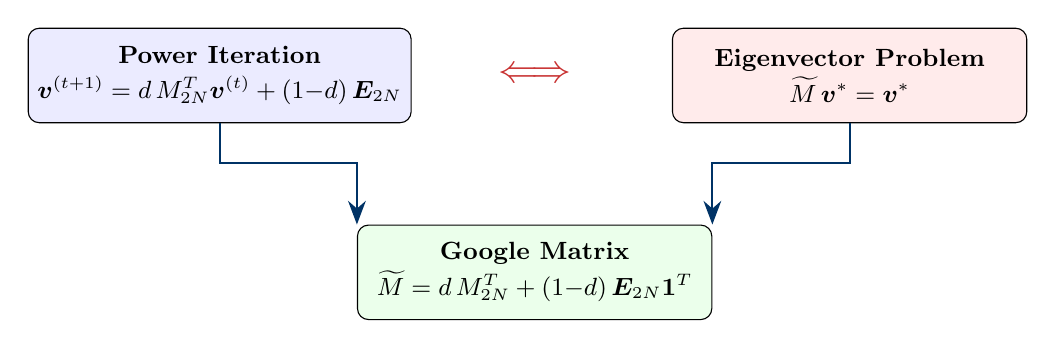
\begin{tikzpicture}[
  box/.style={draw, rounded corners, minimum width=4.5cm, minimum height=1.2cm,
              align=center, font=\small},
  arr/.style={-{Stealth[length=3mm]}, thick, darkblue},
  eq/.style={font=\Large\bfseries, accent}
]

% Left: Power Iteration view
\node[box, fill=blue!8] (pi) at (-4, 0) {
  \textbf{Power Iteration}\\[2pt]
  $\bm{v}^{(t+1)} = d\,M_{2N}^T\bm{v}^{(t)} + (1{-}d)\,\bm{E}_{2N}$
};

% Right: Eigenvector view
\node[box, fill=red!8] (ev) at (4, 0) {
  \textbf{Eigenvector Problem}\\[2pt]
  $\widetilde{M}\,\bm{v}^* = \bm{v}^*$
};

% Equivalence
\node[eq] at (0, 0) {$\Longleftrightarrow$};

% Bottom: Google Matrix
\node[box, fill=green!8] (gm) at (0, -2.5) {
  \textbf{Google Matrix}\\[2pt]
  $\widetilde{M} = d\,M_{2N}^T + (1{-}d)\,\bm{E}_{2N}\bm{1}^T$
};

\draw[arr] (pi.south) -- ++(0,-0.5) -| (gm.north west);
\draw[arr] (ev.south) -- ++(0,-0.5) -| (gm.north east);

\end{tikzpicture}
\end{center}

%======================================================================
\section{Conclusion}
%======================================================================

The Two-Phase PageRank model admits two mathematically equivalent
formulations:

\begin{enumerate}
  \item \textbf{Iterative}: Repeatedly apply $\bm{v} \leftarrow
        d\,M_{2N}^T\bm{v} + (1-d)\,\bm{E}_{2N}$ until convergence.
  \item \textbf{Spectral}: Find the principal eigenvector (eigenvalue
        $\lambda = 1$) of the Google Matrix
        $\widetilde{M} = d\,M_{2N}^T + (1-d)\,\bm{E}_{2N}\bm{1}^T$.
\end{enumerate}

Both yield \emph{exactly the same} stationary distribution $\bm{v}^*$.
The power iteration is preferred because it exploits the sparsity of
$M_{2N}$ and never materializes the dense Google Matrix, reducing
memory from $\sim$300\,GB to $\sim$50\,MB and computation time from
years to seconds.

\end{document}
